\section{Common Algorithms}

\subsection{Noise Generation}
\label{section:noise-generation}
Nature's unpredictability plays a big role in the diversity and appearance of cloudscapes. In shaders, an approach to that \textit{randomness} is used called \textit{\gls{noisegeneration}}.
In order to be able to implement random \gls{noisegeneration}, several important topics need to be looked into. It is best to start with randomness in computer science and how it is handled inside a shader program.

\subsubsection{Random Numbers}
Unfortunately, there is no magic function which returns a pure random number inside the seemingly predictable and rigid code environment.
So the question arises as to how such randomness can be generated.
\\
For this, the function $rnd(x) = fract(sin(x))$ is inspected, where $fract(x) = x - floor(x)$.

\begin{figure}[H]
    \centering
    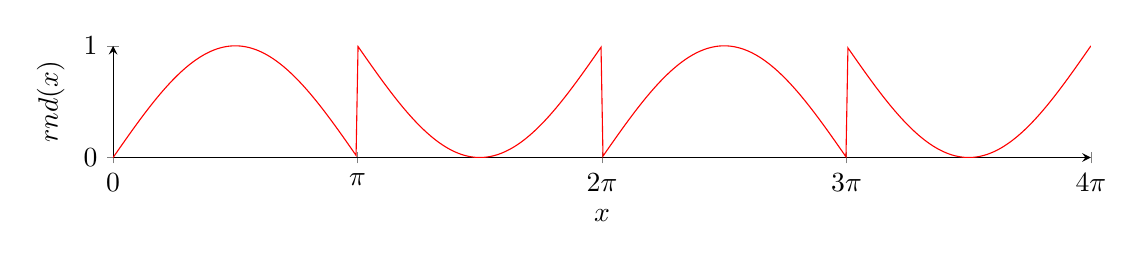
\begin{tikzpicture}[scale=1.0]
        \begin{axis}[
            samples=500,
            domain=0:4*pi,
            axis lines=left,
            xlabel=$x$,
            ylabel={$rnd(x)$},
            height=3cm,
            width=14cm,
            ytick={0,1},
            xtick={0,pi,2*pi,3*pi,4*pi},
            xticklabels={$0$,$\pi$,$2\pi$,$3\pi$,$4\pi$}
            ]
        \addplot[red] plot (\x, { sin(\x*1 r) - floor(sin(\x*1 r)) });
        \end{axis}
    \end{tikzpicture}
    \caption{Random numbers with the fractional value of sine of x.}
\end{figure}

\noindent
The sine values fluctuate between $-1.0$ and $1.0$, but with $fract$, only the fractional part is evaluated, turning the negative values into positive ones.
This effect can be used to get some pseudo-random values by "compressing" the function horizontally, or in other words by increasing the frequency of the sine wave.
\\
The next figure displays the function $rnd(x) = fract(sin(x) * 10000)$.

\begin{figure}[H]
    \centering
    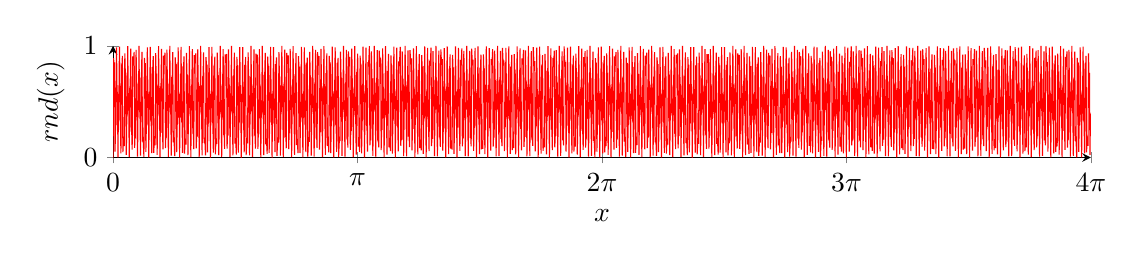
\begin{tikzpicture}[scale=1.0]
        \begin{axis}[
            samples=2000,
            domain=0:4*pi,
            axis lines=left,
            xlabel=$x$,
            ylabel={$rnd(x)$},
            height=3cm,
            width=14cm,
            ytick={0,1},
            xtick={0,pi,2*pi,3*pi,4*pi},
            xticklabels={$0$,$\pi$,$2\pi$,$3\pi$,$4\pi$},
            ]
        \addplot[red] plot (\x, { sin(\x*10000) - floor(sin(\x*10000)) });
        \end{axis}
    \end{tikzpicture}
    \caption{Random numbers with the fractional value of sine of x multiplied by 10000.}
\end{figure}

\noindent
It is clearly visible that the function $rnd(x)$ became chaotic and returns practically random values. However, it is noteworthy that $rnd(x)$ is still a deterministic function, which means for example $rnd(1.0)$ is always going to return the same value.

\clearpage
\subsubsection{2D Random}
To generate a pseudo-random number from two values instead of one, the same function can be used, with some tweaks. Those two numbers come as a two-dimensional vector, which needs to be transformed into a single floating point number.
According to Vivo, the dot product is particularily helpful in that case \cite{online:thebookofshaders}. It returns a single float value between $0.0$ and $1.0$ depending on the alignment of two vectors.
They describe the following method:

\begin{lstlisting}[language=HLSL, caption=Implementation of 2D random number generation., label=lst:random:2d]
float random2d(float2 co) {
    return fract(sin(dot(co, float2(12.9898,78.233))) * 43758.5453123);
}
\end{lstlisting}

\noindent
When using the fragment coordinates as the vector \lstinline[language=HLSL]{co} to call \lstinline[language=HLSL]{random2d(co)} for every pixels, the resulting image shows a seemingly random assortment of pixels holding values from 0 to 1 (from black to white).

\begin{figure}[H]
    \centering
            \includegraphics[width=0.45\linewidth]{noise/2d random}
            \captionof{figure}{2D random function visualized.}
            \label{img:noise:2d:random}
\end{figure}

\noindent
This method of procedural randomness still has one major flaw: It has no patterns. Contratictory to the word \textit{random}, a certain pattern is required in order to generate \textit{random} clouds. Luckily, there is more to random generation than just a highly sped up sine wave.

\clearpage
\subsubsection{Procedural Noise Patterns}
Now that the concept of random numbers in the world of shaders is no longer a mystery, more advanced noise generation algorithms can be introduced.
When using the word \textit{\gls{noise}} in this context, usually procedural pattern generation is meant.

\paragraph{Perlin Noise}
One of the most commonly used procedural pattern generation algorithms is that of Ken Perlin. Named after him, the algorithm works with the gradient, which was already introduced in \sectionref{section:rendering:surfacenormalestimation}.
\\
It consists of the following three steps: 
\begin{itemize}
    \item Grid definition
    \item Dot product calculation between random gradient and distance vectors
    \item Interpolation of those dot product values
\end{itemize}

First, the 2D image space is split into a grid. For each vertex or corner point on this grid, a pseudo-random gradient vector is determined.

\begin{figure}[H]
    \centering
        \begin{minipage}{0.47\linewidth}
            \begin{tikzpicture}[scale=0.8, x=2cm,y=2cm]
                \tikzset{c/.style = {shorten <=-4pt, shorten >=-4pt}}
                \tikzset{smalledge/.style = {-{Latex[length=2mm]},shorten <=-4pt}}
              
                \node (x1y1) at (0,0) {\textbullet};
                \node (x2y1) at (1,0) {\textbullet};
                \node (x3y1) at (2,0) {\textbullet};
                \node (x4y1) at (3,0) {\textbullet};
        
                \node (x1y2) at (0,1) {\textbullet};
                \node (x2y2) at (1,1) {\textbullet};
                \node (x3y2) at (2,1) {\textbullet};
                \node (x4y2) at (3,1) {\textbullet};
        
                \node (x1y3) at (0,2) {\textbullet};
                \node (x2y3) at (1,2) {\textbullet};
                \node (x3y3) at (2,2) {\textbullet};
                \node (x4y3) at (3,2) {\textbullet};
        
                \node (x1y4) at (0,3) {\textbullet};
                \node (x2y4) at (1,3) {\textbullet};
                \node (x3y4) at (2,3) {\textbullet};
                \node (x4y4) at (3,3) {\textbullet};
        
                \draw[c] (x1y1) edge node{} (x4y1);
                \draw[c] (x1y2) edge node{} (x4y2);
                \draw[c] (x1y3) edge node{} (x4y3);
                \draw[c] (x1y4) edge node{} (x4y4);
        
                \draw[c] (x1y1) edge node{} (x1y4);
                \draw[c] (x2y1) edge node{} (x2y4);
                \draw[c] (x3y1) edge node{} (x3y4);
                \draw[c] (x4y1) edge node{} (x4y4);
        
                % arrows
                \draw[smalledge, red] (x1y1) edge node{} ($ (x1y1) + (-0.6,0.2) $);
                \draw[smalledge, red] (x2y1) edge node{} ($ (x2y1) + (0.4,0.4) $);
                \draw[smalledge, red] (x3y1) edge node{} ($ (x3y1) + (0.3,-0.5) $);
                \draw[smalledge, red] (x4y1) edge node{} ($ (x4y1) + (0.5,-0.3) $);
        
                \draw[smalledge, red] (x1y2) edge node{} ($ (x1y2) + (0.3,-0.5) $);
                \draw[smalledge, red] (x2y2) edge node{} ($ (x2y2) + (0.2,0.6) $);
                \draw[smalledge, red] (x3y2) edge node{} ($ (x3y2) + (0.6,-0.2) $);
                \draw[smalledge, red] (x4y2) edge node{} ($ (x4y2) + (0.3,-0.5) $);
        
                \draw[smalledge, red] (x1y3) edge node{} ($ (x1y3) + (-0.3,0.5) $);
                \draw[smalledge, red] (x2y3) edge node{} ($ (x2y3) + (-0.3,-0.5) $);
                \draw[smalledge, red] (x3y3) edge node{} ($ (x3y3) + (0.5,-0.3) $);
                \draw[smalledge, red] (x4y3) edge node{} ($ (x4y3) + (0.5,0.3) $);
        
                \draw[smalledge, red] (x1y4) edge node{} ($ (x1y4) + (0.3,0.5) $);
                \draw[smalledge, red] (x2y4) edge node{} ($ (x2y4) + (-0.1,-0.7) $);
                \draw[smalledge, red] (x3y4) edge node{} ($ (x3y4) + (-0.4,0.4) $);
                \draw[smalledge, red] (x4y4) edge node{} ($ (x4y4) + (-0.3,0.5) $);
        
                \end{tikzpicture}
                \caption{Perlin grid with pseudo-random gradient vectors.}
                \label{img:tikz:noise:gradient}
        \end{minipage}
    \hfill
    \begin{minipage}{0.47\linewidth}
        \begin{tikzpicture}[scale=0.8, x=2cm,y=2cm]
            \tikzset{c/.style = {shorten <=-4pt, shorten >=-4pt}}
            \tikzset{smalledge/.style = {-{Latex[length=2mm]},shorten <=-4pt}}

            \begin{scope}
                \clip (0,0) rectangle (3,3);
                
                \node [shading=axis,rectangle,left color=white, right color=gray,shading angle=180+65,  minimum width=0.8*2cm, minimum height=0.8*2cm] (box) at (x1y1){};
                \node [shading=axis,rectangle,left color=white, right color=gray,shading angle=180-40,  minimum width=0.8*2cm, minimum height=0.8*2cm] (box) at (x2y1){};
                \node [shading=axis,rectangle,left color=white, right color=gray,shading angle=180-145, minimum width=0.8*2cm, minimum height=0.8*2cm] (box) at (x3y1){};
                \node [shading=axis,rectangle,left color=white, right color=gray,shading angle=180-110, minimum width=0.8*2cm, minimum height=0.8*2cm] (box) at (x4y1){};
                
                \node [shading=axis,rectangle,left color=white, right color=gray,shading angle=180-145, minimum width=0.8*2cm, minimum height=0.8*2cm] (box) at (x1y2){};
                \node [shading=axis,rectangle,left color=white, right color=gray,shading angle=180-10,  minimum width=0.8*2cm, minimum height=0.8*2cm] (box) at (x2y2){};
                \node [shading=axis,rectangle,left color=white, right color=gray,shading angle=180-100, minimum width=0.8*2cm, minimum height=0.8*2cm] (box) at (x3y2){};
                \node [shading=axis,rectangle,left color=white, right color=gray,shading angle=180-165, minimum width=0.8*2cm, minimum height=0.8*2cm] (box) at (x4y2){};
                
                \node [shading=axis,rectangle,left color=white, right color=gray,shading angle=180+30,  minimum width=0.8*2cm, minimum height=0.8*2cm] (box) at (x1y3){};
                \node [shading=axis,rectangle,left color=white, right color=gray,shading angle=180+140, minimum width=0.8*2cm, minimum height=0.8*2cm] (box) at (x2y3){};
                \node [shading=axis,rectangle,left color=white, right color=gray,shading angle=180-120, minimum width=0.8*2cm, minimum height=0.8*2cm] (box) at (x3y3){};
                \node [shading=axis,rectangle,left color=white, right color=gray,shading angle=180-55,  minimum width=0.8*2cm, minimum height=0.8*2cm] (box) at (x4y3){};

                \node [shading=axis,rectangle,left color=white, right color=gray,shading angle=180-30,  minimum width=0.8*2cm, minimum height=0.8*2cm] (box) at (x1y4){};
                \node [shading=axis,rectangle,left color=white, right color=gray,shading angle=180+175, minimum width=0.8*2cm, minimum height=0.8*2cm] (box) at (x2y4){};
                \node [shading=axis,rectangle,left color=white, right color=gray,shading angle=180+45,  minimum width=0.8*2cm, minimum height=0.8*2cm] (box) at (x3y4){};
                \node [shading=axis,rectangle,left color=white, right color=gray,shading angle=180+35,  minimum width=0.8*2cm, minimum height=0.8*2cm] (box) at (x4y4){};
            \end{scope}
            
            \node (x1y1) at (0,0) {\textbullet};
            \node (x2y1) at (1,0) {\textbullet};
            \node (x3y1) at (2,0) {\textbullet};
            \node (x4y1) at (3,0) {\textbullet};
    
            \node (x1y2) at (0,1) {\textbullet};
            \node (x2y2) at (1,1) {\textbullet};
            \node (x3y2) at (2,1) {\textbullet};
            \node (x4y2) at (3,1) {\textbullet};
    
            \node (x1y3) at (0,2) {\textbullet};
            \node (x2y3) at (1,2) {\textbullet};
            \node (x3y3) at (2,2) {\textbullet};
            \node (x4y3) at (3,2) {\textbullet};
    
            \node (x1y4) at (0,3) {\textbullet};
            \node (x2y4) at (1,3) {\textbullet};
            \node (x3y4) at (2,3) {\textbullet};
            \node (x4y4) at (3,3) {\textbullet};
    
            \draw[c] (x1y1) edge node{} (x4y1);
            \draw[c] (x1y2) edge node{} (x4y2);
            \draw[c] (x1y3) edge node{} (x4y3);
            \draw[c] (x1y4) edge node{} (x4y4);
    
            \draw[c] (x1y1) edge node{} (x1y4);
            \draw[c] (x2y1) edge node{} (x2y4);
            \draw[c] (x3y1) edge node{} (x3y4);
            \draw[c] (x4y1) edge node{} (x4y4);
    
            % arrows
            \draw[smalledge, red] (x1y1) edge node{} ($ (x1y1) + (-0.6,0.2) $);
            \draw[smalledge, red] (x2y1) edge node{} ($ (x2y1) + (0.4,0.4) $);
            \draw[smalledge, red] (x3y1) edge node{} ($ (x3y1) + (0.3,-0.5) $);
            \draw[smalledge, red] (x4y1) edge node{} ($ (x4y1) + (0.5,-0.3) $);
    
            \draw[smalledge, red] (x1y2) edge node{} ($ (x1y2) + (0.3,-0.5) $);
            \draw[smalledge, red] (x2y2) edge node{} ($ (x2y2) + (0.2,0.6) $);
            \draw[smalledge, red] (x3y2) edge node{} ($ (x3y2) + (0.6,-0.2) $);
            \draw[smalledge, red] (x4y2) edge node{} ($ (x4y2) + (0.3,-0.5) $);
    
            \draw[smalledge, red] (x1y3) edge node{} ($ (x1y3) + (-0.3,0.5) $);
            \draw[smalledge, red] (x2y3) edge node{} ($ (x2y3) + (-0.3,-0.5) $);
            \draw[smalledge, red] (x3y3) edge node{} ($ (x3y3) + (0.5,-0.3) $);
            \draw[smalledge, red] (x4y3) edge node{} ($ (x4y3) + (0.5,0.3) $);
    
            \draw[smalledge, red] (x1y4) edge node{} ($ (x1y4) + (0.3,0.5) $);
            \draw[smalledge, red] (x2y4) edge node{} ($ (x2y4) + (-0.1,-0.7) $);
            \draw[smalledge, red] (x3y4) edge node{} ($ (x3y4) + (-0.4,0.4) $);
            \draw[smalledge, red] (x4y4) edge node{} ($ (x4y4) + (-0.3,0.5) $);
    
            \end{tikzpicture}
            \caption{Perlin grid with visualized gradient vectors.}
            \label{img:tikz:noise:gradient_visualized}
    \end{minipage}
\end{figure}



